\documentclass[output=paper]{langsci/langscibook} 
\ChapterDOI{10.5281/zenodo.2579041}
\author{Krasimir Angelov \affiliation{University of Gothenburg}}
\title{Multiword expressions in multilingual applications within the Grammatical Framework} 


%\lehead{}
\shorttitlerunninghead{Multi-word expressions within the Grammatical Framework}

% \abstract{This chapter is about the Grammatical Framework and 
% how multiword expressions are represented in the framework.
% The main strength of the framework is in multilingual applications
% which also means that multiword expressions are considered
% from a cross-lingual perspective.}

\abstract{The main focus of Grammatical Framework (GF) is in
multilingual applications where the same type of content is
produced and analyzed in several languages at once. This
is achieved by joining the grammars for all languages with
a shared interlingual representation. In designing the interlingua,
multiword expressions are an important factor that must be considered.
Here, I adopt the broader definition where everything that translates
non-compositionally accross languages is considered 
an expression. In this chapter I present multiword expressions
from a cross-lingual perspective in relation to an interlingual
grammar.}

\maketitle

\usepackage{subcaption}

\begin{document}

\section{Introduction}

Grammatical Framework (\isi{GF}, \citealt{ranta-2011}) is a programming language 
for developing multilingual applications. The typical applications are in
natural language generation, dialogue systems, machine translation
or in question answering systems where it is feasible to assume 
a limited language domain. In these scenarios it is possible to design
a controlled language which can be completely covered with
a formal \isi{grammar}. On the other hand, these applications are typically
highly multilingual. It is not uncommon to have a single \isi{grammar}
which supports simultaneously more than twenty languages.
There are a number of challenges in this kind of application.

First of all, in order to scale to a high number of languages,
GF is designed to work with an interlingua. Every \isi{grammar}
is divided into an abstract syntax and one or more concrete syntaxes.
The abstract syntax is a language-independent interlingual representation
of the application domain, while each of the concrete syntaxes
renders an abstract syntax tree into a string in 
the corresponding natural language. In that setting, translation, for instance,
is reduced to parsing the input sentence into an abstract
tree and then rendering of the same tree into another concrete language.

Furthermore, developing even a small language fragment would normally
require several low-level details, such as word order and gender/number
agreement, to be reimplemented from scratch for every language
and for every application. This would be highly ineffective if
it was not aided by the development of the Resource Grammars Library (RGL, \citealt{gf-rgl}) in \isi{GF}.
RGL is a library of wide coverage grammars for more than thirty 
languages developed by a community of linguists and computer scientists.
By reusing the library, new applications can be built in short time
by people who do not even have to be linguistically trained and who
may not be experts in the target languages.

Working on the level of the RGL is still too low-level though. The
library is trying to hide syntactic differences across languages but
this is still not what we ultimately want in an application.  What is
needed is a model which can abstract over the language-independent
semantics of the sentence. Phenomena like constructions and multiword
expressions translate non-compositionally across languages, and thus
are recurring obstacles that have to be resolved in every
application. For that purpose there is a different \isi{grammar} for
each application. Application grammars, for example, are more
semantically oriented. On the other hand, resource grammars are
syntactic.  Another difference between these two grammars is that
resource grammars are highly lexicalized, but lexical entries often
become semantic functions in application grammars. This is a key
design decision which allows us to have an abstract language-independent
representation. For example, such a representation lets us hide the language-specific
multiword expressions in the modules for the concrete languages,
without affecting the abstract syntax.

This strategy has been proven efficient in limited domains, and most of
this chapter will be about how language-specific multiword expressions
and constructions are represented in GF.

We have recently started to scale up from limited-domain
applications to wide coverage parsing and translation. 
For this to be successful, it is important to have a library
of commonly used constructions across different languages. 
Although this is still a moving target, I will report on the current
efforts to build such a library by either reusing existing resources,
or by creating those using automatic methods.
This also shows that the strategy used for limited
domains can scale to an open domain, when there is a wide-coverage
resource of raw data that can be ported to the platform.

Please note that moving from lexicalized syntactic grammars to unlexicalized semantic grammars requires, for many languages, syntax to be represented in a
discontinuous way. Just to give a simple example, forming questions
in \ili{English} requires that we move or add auxiliary verbs
in front of the sentence, while the rest of the verb \isi{phrase}
is left somewhere in the middle. Other languages might not use
auxiliaries at all or they might just form questions differently.
This means that the verb \isi{phrase} in \ili{English} must be modelled
as a single \isi{phrase} with two discontinuous parts. The implications
from this for the implementation of the framework will be discussed
as well.

\section{The basic principles of GF}

\isi{GF} is designed as a multilingual framework from the ground up.
A typical application starts by identifying the relevant
domain and then describing the desired phrases within that domain
in multiple languages. In order to accommodate and link several
diverse languages, the framework separates the \isi{grammar} into two distinct
conceptual layers: abstract and concrete syntax.

The \textsc{abstract syntax} is a logical framework which acts as a language independent interlingua. It defines a collection of types and functions which can be used to build abstract syntax trees. Each abstract tree represents a \isi{phrase} which is realized by using one of the available \textsc{concrete syntaxes}. In this section, I will informally introduce the abstract and the concrete syntax in \isi{GF} by example. For a more detailed introduction to \isi{GF} we refer to \cite{ranta-2011}.

We start with the lexicon. On an abstract level, the lexicon consists of a simple inventory of word senses. For example, we might have:
\begin{verbatim}
      cat N
      fun horse_N : N
\end{verbatim}
Here the first line declares that there is a category \verb=N=, which will denote the type of all nouns. The second line defines a function with no arguments, a.k.a. a constant of type \verb=N=. These abstract constants serve as cross-lingual lemmas. By convention we use names composed of an \ili{English} lemma followed by a part of speech tag. When these are not sufficient to disambiguate the meaning of the word, then we can add more elements. For example, we could use WordNet's sense numbers for disambiguation:
\begin{verbatim}
     fun arm_1_N : N         (body part)
     fun arm_3_N : N         (weapon)
\end{verbatim}

The lexicon starts to get interesting only when we move to 
the concrete syntax. The concrete syntax for \ili{English} 
looks something like:
\begin{verbatim}
  lincat N = Number => Str
  lin horse_N = table {Sg => "horse" ; Pl => "horses"}
\end{verbatim}
Here the keyword \verb=lincat= introduces the linearization category 
for nouns, i.e. for the type \verb=N=, and \verb=lin= introduces 
the linearization of the function \verb=horse_N= itself.

In programming language parlance, the abstract category \verb=N= 
is like an abstract data type, i.e. a mere name with 
a hidden implementation, while the linearization category in 
the concrete syntax is its actual implementation. 
In \isi{GF}, unlike in other programming languages, a single type 
or a single function might have several different implementations -- 
one for every concrete syntax. In this case, the implementation in 
\ili{English} says that \verb=N= is a table or an array of 
strings (\verb=Str=) indexed by a \verb=Number=. 
The number itself is another data type defined as an enumeration 
with two possible values -- singular (\verb=Sg=) and plural (\verb=Pl=):
\begin{verbatim}
  param Number = Sg | Pl
\end{verbatim}

The linearization of \verb=horse_N=, on the other hand, gives 
the actual values in the table. In \ili{English} these would be 
the word forms \textit{horse} and \textit{horses}, and in 
\ili{French} \textit{cheval}, \textit{chevaux}. In \ili{French}, however, we also need to 
know the gender of the noun in order to take care of 
the word agreement in the syntax. Because of that 
the corresponding definition in the concrete syntax for \ili{French} is slightly
more complicated:
\begin{verbatim}
  lincat N = {s : Number => Str ; g : Gender}
  lin horse_N = 
            {s = table {Sg => "cheval"; Pl => "chevaux"};
             g = Masc
            }

  param Gender = Masc | Fem
\end{verbatim}
Here the linearization category for \verb=N= is not a simple table of 
word forms but a record with two fields -- \verb=s= and \verb=g=. 
The field \verb=s= is still an inflection table like in \ili{English}, 
but there is also the field \verb=g= of type \verb=Gender= with 
two possible values, \verb=Masc= and \verb=Fem=. The linearization 
for \verb=horse_N= assigns to the field \verb=s= the inflection table 
for \ili{French} and sets the field \verb=g= to \verb=Masc=.

It is also possible to have records which combine together more than 
one string field. This is used for instance in \ili{English} 
where \isi{phrasal verbs} consist of a main verb and a particle. 
Those verbs are modelled as records:
\begin{verbatim}
  lincat V2        = {s : VForm => Str; part : Str; prep : Str}
  lin swith_off_V2 = {s = table {VInf =>"switch";
                                 VPres=>"switches";
                                 ...};
                      part = "off"
                      prep = ""}
\end{verbatim}
The field \verb=part= keeps the particle while the \verb=s= field is the inflection table of the main verb. There is also a third field, \verb=prep=, which stores the potential preposition for transitive verbs. Since there is no preposition in this case, an empty string is added. In \isi{prepositional verbs}, however, this field will be non-empty. It is even possible to have verbs with both a particle and a preposition.

It is possible to have multiple string fields in nouns as well. This happens for instance in Chinese where a noun is characterized by its lemma and its classifier. Both are string fields and they could be arbitrarily far apart in the final sentence. For that reason they are stored as two different fields in the record:
\begin{verbatim}
  lincat N = {s : Str; c : Str}
  lin horse_N = {s = "ma"; c = "pi"}
\end{verbatim}

The structure of the lexicon in all languages is 
conceptually very similar. There might be more numbers and genders, 
or there might be grammatical cases, but in general a \isi{lexical entry} in 
\isi{GF} is an inflection table indexed by one or more parameters, and 
there might be additional fields for features such as gender, 
word class, classifier, or a particle. 

The records shown above are rarely what 
the \isi{GF} grammarian actually writes. Instead it is possible to 
isolate common patterns into reusable operations which allow us to 
have succinct definitions like:
\begin{verbatim}
  lin horse_N = mkN "horse" ;
  lin switch_off_V2 = mkV2 (partV (mkV "switch") "off");
\end{verbatim}
Here the smart paradigm \citep{dblp:conf/eacl/detrezr12} operations 
\verb=mkN= and \verb=mkV= are responsible for predicting 
the inflection tables of nouns and verbs from the lemma. 
When the inflection is not predictable from the lemma alone then 
it is possible to specify extra arguments, i.e.:
\begin{verbatim}
  lin mouse_N = mkN "mouse" "mice";
\end{verbatim}
In this case the second argument of \verb=mkN= is 
the irregular plural form of \textit{mouse}. Auxiliary operations 
like \verb=partV= and \verb=mkV2= are used to set the particle or 
the transitivity of the verb.

Having set the basics of the lexicon we can move on to the syntax. 
In the abstract syntax, the syntax is represented as a collection of 
n-ary functions. For example, adjectival modification requires two 
functions, \verb=AdjCN= and \verb=UseN=:
\begin{verbatim}
  cat AP; CN
  fun AdjCN : AP -> CN -> CN
  fun UseN : N -> CN
\end{verbatim}
This yields to two syntactic categories: adjectival phrases (\verb=AP=) and 
common nouns (\verb=CN=). The simplest common noun consists of just 
a single noun (\verb=N=) and is produced by the function \verb=UseN=. 
The function \verb=AdjCN= lets us to modify the noun with one or 
more adjectival phrases. How exactly the adjectival phrases are
attached is language specific.

In \ili{English}, there is no gender and the adjective is always before the noun. The linearizations for \verb=AdjCN= and \verb=UseN= are simply:
\begin{verbatim}
  lincat AP = Str
  lincat CN = Number => Str

  lin UseN n = n
  lin AdjCN ap cn = table {Sg => ap ++ cn ! Sg;
                           Pl => ap ++ cn ! Pl}
\end{verbatim}
Note that when building common noun phrases it is still not known whether 
the \isi{phrase} should be used in singular or in plural. It will remain unknown
until a determiner is fixed and a complete noun \isi{phrase} built. 
For that purpose, the linearization category for \verb=CN= is 
an inflection table indexed by number just like for the 
\verb=N= category. Since the linearizations for 
\verb=CN= and \verb=N= are the same, the linearization rule for 
\verb=UseN= is just the identity function. Since I have defined 
the linearization for adjectives to be a plain string, 
the linearization for \verb=AdjCN= simply concatenates 
the adjective \isi{phrase} in front of the common noun. Here the \verb=(++)=
operator indicates concatenation of token sequences, and 
the exclamation mark \verb=(!)= is used to fetch the element 
from the table that corresponds to a given parameter.

Note that the two elements in the table of the last example are identical
except that they select different numbers. There is a handy shorthand
notation for this case:
\begin{verbatim}
  lin AdjCN ap cn = \\n => ap ++ cn ! n
\end{verbatim}
Here the operator \verb=(\\)= creates a table whose index is the variable
\verb=n=. After the double arrow \verb/(=>)/ is the value itself, 
which is defined by using the variable \verb=n=. When I
substitute \verb=n= with \verb=Sg= and \verb=Pl= I get the same values
as in the previous example.

In \ili{French}, the adjectival modification requires gender and number agreement. 
In addition, the adjective is sometimes put before and sometimes after the noun. 
This means that we need a more complex linearization type for \verb=AP=:
\begin{verbatim}
  lincat AP = {s : Gender => Number => Str;
               isPrefix : Bool}
\end{verbatim}
This type consists of an inflection table for the adjective and a Boolean parameter which determines whether the adjective should be placed before or after the noun. The linearization rule for \verb=AdjCN= now is:
\begin{verbatim}
  lincat CN = {s : Number => Str; g : Gender}
  lin AdjCN ap cn = {
    s = \\n => let 
                 aps = ap.s ! cn.g ! n; 
                 cns = cn.s ! n
               in case ap.isPrefix of {
                    True  => aps ++ cns;
                    False => cns ++ aps
                  }
    g = cn.g
    }
\end{verbatim}
Here, in the \verb=let= expression I first compute the right forms of 
the adjective and of the basic common noun. After that, 
I concatenate them in the right order depending on 
the parameter \verb=isPrefix=. Note that \verb=cn.g= 
is used in two different places. First it gives the right gender 
to use for the adjective, and second it is used to propagate 
the gender from the smaller common noun which is an 
argument of \verb=AdjCN= to the bigger \isi{phrase}. 
The rest of the syntax is built in a similar fashion by adding more 
and more syntactic combinators.

This section had the goal to demonstrate
the essential features of \isi{GF} and how these make it possible to 
hide language-specific details. In the abstract syntax I merely 
say that there are adjectives and nouns and that those 
can be combined together. How exactly this happens is determined by 
the concrete syntax. In this way, the abstract syntax 
can stay language-independent while all language-specific features 
can still be handled. It could be rightfully argued that 
the level of abstractness as it is presented so far is still not 
sufficiently high. For example, I still assume that all languages 
have adjectives and nouns, which might be questioned for some languages. 
It did, however, work for the 30+ languages that are already supported 
in the framework. 
% (TODO: It is claimed by some linguists that Chinese and Japanese 
%  doesn’t have adjectives and instead there are stative verbs. 
%  This could be the source of an interesting discussion here. 
%  We still treat those as adjectives in \isi{GF}).
The most important problem that I will address in the next section, 
however, is that what is an adjective, noun, or verb in 
one language might not belong to the same part of speech in another language.
This is a source of non-compositional constructions and 
multiword expressions that need to be handled on a different level 
in the framework.

\section{Constructions and multiword expressions in GF}
\label{ang:mwe}

I shall divide expressions in two non-overlapping classes since 
they are handled differently in \isi{GF}. The first class are expressions 
that have meaning only as a whole and that cannot be understood 
by interpreting their parts compositionally. 
Examples for those are \textit{by and large}, \textit{after all}, 
\textit{long time no see}, \textit{instead of}, \textit{because of}, etc.
Such expressions are composed of smaller units which have 
in general their own semantic and syntactic uses, but inside 
the expressions they are just tokens constituting a larger unit.
MWEs cannot be parsed by using meaningful grammatical rules.
For instance, in order to parse \textit{instead of} compositionally, 
a syntactic rule could be added, which combines an adverb and 
a preposition to form another preposition:
\begin{verbatim}
  fun foo : Adv -> Prep -> Prep
\end{verbatim}
A rule like this would have no other use but to cover controversial 
syntactic sequences which do not have any compositional meaning anyway.
This makes even less sense in a multilingual setting, since the internal
structure of those expressions in \ili{English} does not persist in other
languages. In \ili{Swedish}, for instance, \textit{because of} translates as 
\textit{p{\aa} grund av}, and in \ili{Bulgarian}, \textit{instead of} translates 
as \textit{vmesto}. In both cases the translation is 
another prepositional expression, but its internal composition 
is very different. The solution is very simple: to ignore 
the bogus internal composition of those expressions and to add them as 
multiword units in the lexicon:
\begin{verbatim}
  fun instead_of_Prep, because_of_Prep : Prep
  lin instead_of_Prep = mkPrep "instead of"
  lin because_of_Prep = mkPrep "because of"
\end{verbatim}

The implication of this choice is that the parser in 
\isi{GF} \citep{angelov2011mechanics} has to work, not on the level of words, 
but on a different, more semantic level. In the case of 
multiword expressions, this semantic level is a cross-words level, and, 
in agglutinative languages, it is often a sub-word level \citep{angelov2015orthography}. 
This complication means, for instance, that unlike in
most other statistical parsers, \isi{GF} parsing is not done on top of 
a part of speech tagged input. Instead, the parser performs both parsing
and tagging, where a single tag might span several tokens or 
conversely only a part of a token.

A subclass of non-compositional expressions is the class of phrasal and 
\isi{prepositional verbs}. Examples of those were shown in 
the previous section. The complication in this case is that they are 
not only composed of multiple words but the words are not 
even consecutive. Unlike in frameworks based on context-free grammars, 
in \isi{GF} this is a trivial matter. Discontinuous expressions 
are modelled by simply using more than one string fields inside a record.
On a low-level both tables and records in \isi{GF} are modelled as 
tuples of strings which reduces the formalism to 
a Parallel Multiple Context-Free Grammar (PMCFG, \citealt{seki91:mcfg}) 
which is beyond context-free grammars. When an expression is embedded in 
a sentence, then the syntactic rules know where to put each of 
the constituents. The assumption, however, is that 
all lexical units of the same type have the same types of discontinuities. 
For instance, the linearization type for all two-argument verbs in \ili{English} is:
\begin{verbatim}
  lincat V2 = {s : VForm => Str; part : Str; prep : Str}
\end{verbatim}
However, only some verbs have particles and only some others have prepositions. In a monolingual \isi{grammar} it is possible to split the category into a category for simple verbs and a category for phrasal/\isi{prepositional verbs} but this does not scale across languages. Phrasal verbs in \ili{English}, for example, are often translated to simple verbs in Slavic languages, where the information from the particle is encoded as a prefix attached to the root. Conversely, simple verbs in \ili{English} might become \isi{prepositional verbs} in other languages or vice versa.

The second class of expressions is those that have both a compositional 
and a non-compositional meaning. It is often the case that the second is 
the most frequent meaning but the former cannot be excluded either. 
Since \isi{GF} is a multilingual framework, the most natural way of 
identifying multiword expressions is cross-lingual. If an expression 
has a non-compositional meaning then it is quite likely that 
it will be expressed in a very different way in another language. 
This is a very empirical criterion which makes it easier to detect 
multiword expressions, but on the other hand, it fuses 
multiword expressions with constructions. Basically anything with 
a non-compositional abstract syntax across languages is considered 
a multiword expression. This kind of expressions is obviously a problem 
in an interlingua-based system.

The solution is to identify and factorize expressions. 
Figure \ref{ang:fig:have_name} shows the abstract syntax trees for 
the sentences \textit{My name is John} in \ili{English} and 
the equivalent \textit{Ich hei{\ss}e John} in \ili{German}. 
The translation is non-compositional because \ili{English} has 
no equivalent for the \ili{German} verb \textit{hei{\ss}en}. 
In a transfer-based translation system, I would have to explicitly 
manipulate the trees to get the one from the other. 
In an interlingual system I can factorize. 

We add in the abstract syntax a new function which takes as input 
all fragments from the individual trees that stay invariable. 
In each of the concrete syntaxes we define that the function produces 
the corresponding language specific trees where the invariable subtrees 
are just plugged in the right places. In the particular case we would get:

\begin{description}[labelindent=0cm,leftmargin=0mm]
\item[Abstract:]~
\begin{verbatim}
  fun have_name_Cl  : NP -> PN -> Cl
\end{verbatim}
\item[\ili{English}:]~
\begin{verbatim}
  lin have_name_Cl p n = PredVP (DetCN (PossNP p) (UseN name_N))
                                (UseComp (CompNP (UsePN n)))
\end{verbatim}
\item[\ili{German}:]~
\begin{verbatim}
  lin have_name_Cl p n = PredVP p (CompV2 (mkV "heissen") (UsePN n))
\end{verbatim}
\end{description}

\begin{figure*}
    \centering
    \begin{tabular}{@{}c@{}c@{}c@{}}
       %% 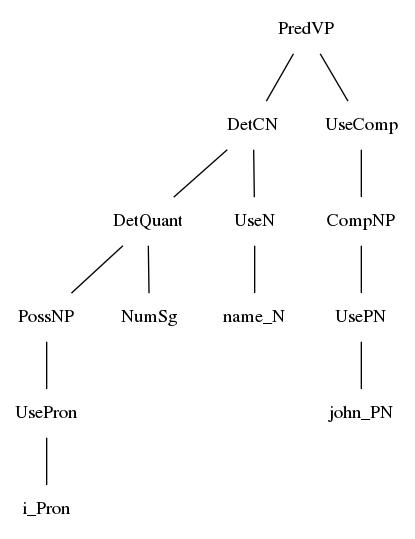
\includegraphics[width=0.35\textwidth]{figures/engname.png} &
       %% 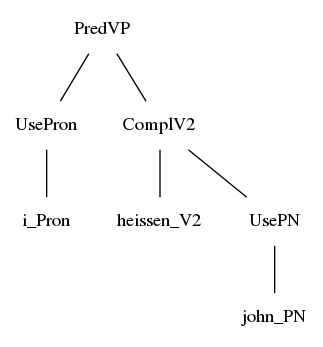
\includegraphics[width=0.35\textwidth]{figures/gername.png} &
       %% 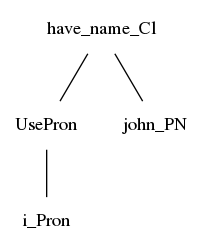
\includegraphics[width=0.2\textwidth]{figures/hasname.png} \\
      {\scriptsize
        \Tree  [.PredVP [.DetCN [.DetQuant [.PossNP [.UsePron i\_Pron ] ] NumSg ] [.UseN name\_N ] ] [.UseComp [.CompNP [.UsePN john\_PN ] ] ] ]}
      &
      {\scriptsize
        \Tree [.PredVP [.UsePron i\_Pron ] [.ComplV2 [heissen\_V2 ] [UsePN john\_PN ] ] ]}
      &
      {\scriptsize
        \Tree [.have\_name\_Cl [.UsePron i\_Pron ] john\_PN ]}
      \\
      a) My name is John &
      b) Ich hei{\ss}e John &
      c) Factorization
    \end{tabular}
    \caption{An example for non-compositional abstract syntax}
   \label{ang:fig:have_name}
\end{figure*}

The new function takes as arguments the subject (\verb=NP=) and 
the proper name (\verb=PN=) and produces a clause (\verb=Cl=).
In the \ili{German} example the subject is actually the pronoun \textit{ich}
with an abstract syntax \verb=UsePron i_Pron=. In \ili{English}, on the
other hand, the syntactic subject is \textit{my name} but we are only
interested in varying \textit{my} so the argument \verb=UsePron i_Pron=
is wrapped with \verb=PossNP= which in \ili{English} generates a possessive determiner
from an \verb=NP=, i.e. from \textit{I} we get \textit{my}. The determiner
is then applied to the noun \textit{name}.
The result is of category clause which is the same as a sentence except that it has 
variable tense and word order. This makes it possible to reuse it for building 
relative clauses, questions and sentences. We can also inflect it 
in tense and polarity. This means that it is enough to factorize 
the construction only once and then it automatically becomes available 
in all possible forms. Once we have the new abstract function then 
we can use a language-independent tree as shown on Figure \ref{ang:fig:have_name}c.

Note that in the linearization rules, unlike in the lexicon and in the syntax of the \isi{grammar}, tables and records were not used. 
Instead we are free to reuse the already existing syntactic functions 
that are available in the \isi{grammar}. In the previous section, 
how to define functions, such as \verb=AdjCN= and \verb=UseN=, was introduced. These functions can be used not only for parsing/generating sentences but also inside the definitions of new functions. This is exactly what is done here and thus, a lot of low-level details can be avoided.

For lexical units we can either reuse existing lexical definitions 
like \verb=name_N= or define locally new ones like \verb=mkV "heissen"=.
This is handy since nouns like \verb=name_N= are more common across 
languages and thus we would probably want them in 
the general lexicon anyway. On the other hand, verbs equivalent to 
\textit{hei{\ss}en} can be found in only some languages.

The previous example can be explained as a construction which differs
across languages because of a lexical gap, i.e. the missing \textit{hei{\ss}en}
verb in \ili{English}. However, exactly the same solution can be also used for
pure \isi{idioms}. For example, a prototypical multiword expression like
\textit{kick the bucket} in \ili{English} can be defined as a lexical verb \isi{phrase}:
\begin{verbatim}
fun kick_the_bucket_VP : VP
lin kick_the_bucket_VP = ComplSlash (SlashV2a kick_V2) 
                                    (DetCN (DetQuant DefArt NumSg)
                                           (UseN bucket_N))
\end{verbatim}
A translation to another language could be realized either as a single
verb equivalent to \textit{die} or as another idiom. In either case
the translation should still function as a verb \isi{phrase}. Note that the
verb \isi{phrase} above is not just a complicated way to encode the string 
\textit{kick the bucket}. When the expression in the example is evaluated
it is reduced to a complex data structure which, among other things, contains
all inflection forms of \textit{kick} as well as all auxiliary verbs that
must be used for forming the different tenses in \ili{English}.

The common feature between the last two examples is that in both
cases we have to move from lexical categories such as noun and verb
to a higher-level syntactic categories. For example instead of assuming
the existence of a specific verb we just assume that there is a specific
verb \isi{phrase} or a sentence that conveys the same meaning. Similarly
instead of nouns we use noun phrases and instead of adjectives -- adjective phrases.
Basically we move upwards in the hierarchy of syntactic categories until
we reach a level where the differences across languages are entirely
contained within the selected category. 

If the multiword expression
contains variable parts then they become arguments of the abstract
syntax function. The order in which the arguments are listed in the
type of the function is completely irrelevant since in the concrete
syntax we are free to use the arguments in an arbitrary order regardless 
of the order in which they are declared. It is just by convention that
we usually choose to use the order in which they are used in \ili{English}.
Note, however, that this freedom does not come for free. 
For instance, most statistical PMCFG parsers assume that 
the arguments to a function are used in the order in which they are defined.
This assumption is always satisfiable if the \isi{grammar} is monolingual but in 
a multilingual setting there is simply no natural order. Moreover,
the \isi{grammar} in a typical statistical parser is learned from corpora
and is generally not intended to be interpreted, so any argument order
is just as good. In contrast the typical \isi{GF} \isi{grammar}
is developed by a grammarian who might have his/her own aesthetic
preferences.

Using functions with arguments is just one of the ways to make
a multiword expression variable. Sometimes general modifiers 
are admitted in the middle of an expression.
Typical examples are light verb constructions such as \textit{I am back}
which also admit modifications like \textit{I am \textbf{already} back}.
It is not difficult to model the verb \isi{phrase} \verb=copula+back=:
\begin{verbatim}
  lin am_back_VP = UseComp (CompAdv back_Adv)
\end{verbatim}
What is not visible here, however, is that the computed verb \isi{phrase}
is discontinuous. The two important parts are an inflection table with
all forms of the copula and a second field which contains the argument
of the copula, i.e.\ the adverb \textit{back}. 
Now if we modify the new lexical verb \isi{phrase}:
\begin{verbatim}
  AdVVP already_AdV am_back_VP
\end{verbatim}
then the Resource Grammar automatically knows that the adverb
\textit{already} should be inserted between the copula and the argument.
The insertion is possible only because of the discontinuity of 
the verb \isi{phrase}. Note also that the same adverbial modification in another
language may not require discontinuity. For example the equivalent in
\ili{Bulgarian} for \textit{I am back} consists of a single verb and then 
the adverb is placed before the verb. None of this, however, is
visible in the abstract syntax.

In general the ability of the framework to deal with discontinuous phrases
is heavily exploited in the resource \isi{grammar}. It is one of the most powerful
features that allows us to hide language specific details and it helps
in the implementation of some constructions.

\section{Libraries of constructions in GF}

Constructions and multiword expressions are really abundant in 
any natural language, and it is part of our mission to collect and 
organize \isi{GF} resources for as many languages as possible. The main
realization of that mission, so far, is the RGL.
In the recent years we have also started to collect general lexical
resources. Ultimately we would like to have a Resource Lexicons Library
with a multilingual translation lexicon for many languages.
Even that is not the end and we should also consider collecting libraries
of constructions. There were two pilot projects in that direction:
\cite{gruzitis2015formalising} and \cite{enache2014handling}.
 
In \cite{gruzitis2015formalising} the goal is to formalize the
\ili{Swedish} Constructicon \citep{konvens:lyngfelt12w}. 
The original constructicon is a semi-formal 
database which covers common constructions in \ili{Swedish} relevant for
second language learners. There is also an ongoing work to link 
the resource with the Berkeley Constructicon for \ili{English} \citep{backstrom}. The focus,
however, is in language learning rather than parsing or translation.
As such it was not the primary goal to organize the constructicon as
a formal \isi{grammar} usable for automatic processing. Instead each entry
in the resource combines an informal textual description with 
a syntactic pattern written in a semi-formal style. 
The syntactic patterns were parsed and converted to \isi{GF} rules
which extend the \ili{Swedish} Resource Grammar.

The original constructicon contains 374 entries of which the project
focused on the 105 constructions for verb phrases. Due to inconsistencies
in the original resource in the first round only 43 out of 
the 105 constructions were successfully converted. 
After several iterations of manual inspection and correction, 
the number of successful constructions increased to 93. The remaining
cases were consistently annotated but are corner cases that are currently
not supported by the conversion algorithm. The necessary corrections
and inconsistencies were sent back to the developers of the constructicon
and are fixed by now. The experiment, however, clearly showed the advantage
of using a formal system that can guard against accidental errors
that are imminent in a free text format.

At the end each of the constructions was converted to one or 
more \isi{GF} functions which in total resulted in 127 abstract functions. 
For 98 out of these 127 abstract functions, the corresponding 
concrete syntax was also successfully constructed automatically.
A logical continuation of the project would be to also convert the
aligned entries from the Berkeley Constructicon and later
to add other languages.

\cite{enache2014handling} started from a much lower level and tried
to find candidates for multiword expressions from 
the Wikitravel \isi{phrase} collection
in \ili{English}, \ili{German}, \ili{French} and \ili{Swedish}. The general idea is that,
given a pair of parallel sentences, the algorithm extracts all
possible abstract syntax trees for each sentence and if there
is no common abstract tree for both sentences, then the pair must
contain a non-compositional expression. The candidates are then
manually examined and the new constructions are added in a library
of constructions. The majority of constructions found in this way
span over larger syntactic structures and are thus above the level of
a simple lexicon. For example out of 171 candidates 142 expressions
were syntactic. They can be roughly classified as: greetings, weather
reports, time expressions, money, units of measurement and spatial deixis.
The remaining 29 expressions are lexical. For example \textit{locker}
in \ili{English} translates as \textit{l{\aa}sbart sk{\aa}p} (`lockable closet')
in \ili{Swedish}.

Another experiment in \cite{enache2014handling} is to learn
a lexicon of compound nouns between \ili{English} and \ili{German}. The method
uses automatic \isi{word alignment} in a parallel corpus. The candidates for
compounds are pairs of phrases where: the \ili{English} side must be parsable
as a noun \isi{phrase} with the \isi{GF} \isi{grammar}, the \ili{German} side must consist
of a single word, and finally the overall probability for the pair must
be above a fixed threshold level. The compound nouns extracted in this
way were added to the lexicon of a \isi{statistical machine translation}
system and the evaluation showed a noticeable improvement in the BLEU
score.

\section{Application grammars}

The discussions so far were on the level of the Resource Grammars.
The typical \isi{GF} applications, however, never use the resource grammars
directly. Instead they are used as libraries to build application grammars.
The main difference is that while the abstract syntax of a resource \isi{grammar}
describes some kind of abstracted syntactic level, the application
\isi{grammar} describes an abstracted domain semantics. Another way to see
the difference is to think about the abstract syntax of the application grammar as an ontological
language for describing the application domain. The abstract syntax
of the resource \isi{grammar}, on the other hand, is an ontology which describes
the syntactic constructions that someone would expect to find in a natural
language.

While in the resource \isi{grammar} we work with categories like noun \isi{phrase}
and verb \isi{phrase}, in the application \isi{grammar} we switch to semantic
categories like person, agent, food, drink, etc. The abstract syntax
functions, on the other hand, are semantic predicates which take, for instance,
an agent and a drink and produce a statement like:\\[10pt]
%
{\phantom{X}\qquad\qquad \textit{someone\texttt{(person)} drinks something\texttt{(drink)}}}\\[10pt]
%
The main role of these new semantic categories is to provide 
sortal restrictions on the types of nouns that can be used for the
different arguments of the predicates. Otherwise the predicates are
implemented in a fashion that is very similar to the one for
multiword expressions presented in Section \ref{ang:mwe}.
In particular most of the predicates are de-lexicalized which
gives us more freedom to keep the abstract syntax language-independent
while hiding all differences in the concrete syntax. 

The sortal restrictions might be relevant for general
multiword expressions as well. For example part of the
annotations in the \ili{Swedish} Constructicon are about semantic roles
such as \texttt{Actor}, \texttt{Theme}, \texttt{Result}, etc.
Those were ignored while converting the resource to \isi{GF}, but
it is possible that some of these constructions are valid only when
the constraints are satisfied.

There are several advantages in working with application grammars.
First, they are typically much smaller than the resource grammars, which
also makes them computationally much more efficient. Second, since
the application grammars cover only a specific domain, they can
guarantee translation with publishing quality. However, when the resource
grammars are used directly in translation then the quality is much worse.
Most of the problems can be attributed to multiword expressions
which are simply not covered by the vanilla resources. 
Having a comprehensive \isi{grammar} of multiword expressions should
improve the quality a lot, but since building 
a general and comprehensive resource is very expensive, we currently
do it on application by application basis.

The main disadvantage of the application grammars is that they lack
robustness. They can analyse input conforming to the \isi{grammar} but
fail completely if there is even a minor violation. For that reason
they are mostly used for controlled languages 
\citep{angelov:2009:icl} where the users must use 
authoring tools that help them to stay within the scope of the \isi{grammar}.
A screenshot of one of those tools \citep{ranta2010tools}
is shown on Figure \ref{ang:fig:fridge}. With this interface the users
are not allowed to enter free text but instead they compose a sentence
by choosing words from a list of options. The sentence is built
incrementally and at each step the list contains only words
that are permitted as a possible next word in the sentence.

\begin{figure}
\center
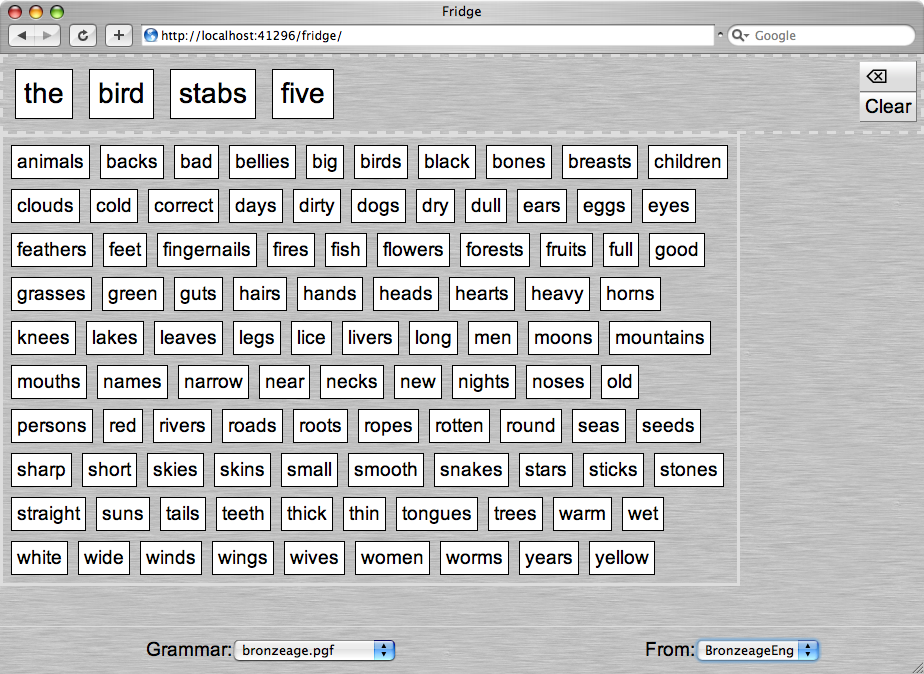
\includegraphics[width=0.9\textwidth]{figures/fridge-poetry-screenshot}
\caption{An authoring interface for writing Controlled Languages}
\label{ang:fig:fridge}
\end{figure}

The controlled language authoring is useful only when the \isi{grammar}
is restrictive. If the same interface is used with the resource \isi{grammar},
then since there are very little restrictions, almost every word can
appear almost everywhere. The analysis of a strange combination of words,
however, could be equally strange. The other disadvantage of that 
interface is that it is not possible to get an overview of 
all constructions that are available in the \isi{grammar}. In a sense, that
interface gives us the ant's point of view which sees each word
one by one. What we sometimes want is the bird's view which sees the
\isi{grammar} from the top. 

One such interface was developed in \cite{parlira}. With that interface 
the user is first presented with a list of all possible constructions. 
When a particular construction is chosen then he/she is guided to 
a customization interface
like the one on Figure \ref{ang:fig:parlira}. There the user sees an example
of the construction rendered in two languages. Below the example,
there is a list of options that can be used to customize the construction.
On the figure, the example is the construction is \verb=have_name_Cl= from
Section \ref{ang:mwe} rendered in \ili{Swedish} and \ili{Bulgarian}. The possible
customizations are to turn the construction from a statement to a question
or to change the subject, i.e.\ \textit{Who are we talking about?}.

\begin{figure}
\center
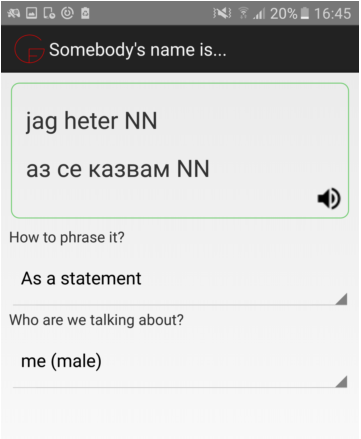
\includegraphics[width=0.35\textwidth]{figures/parlira1}
\caption{A browsing interface for an application grammar}
\label{ang:fig:parlira}
\end{figure}

This particular interface is not restricted to controlled languages.
It can be configured to work with any \isi{grammar} where the configuration
describes which phrases should be included in the browser.
For example, if it is coupled with the resource \isi{grammar}, then it
is not necessary to make the whole of the \isi{grammar} visible.
Instead the browser can only include phrases that are relevant
for a particular purpose. For example, the interface is currently used
in an offline mobile translation application \citep{angelov:android}
which can translate free text. The browsing interface, however,
does not expose the entire \isi{grammar}, and instead it only
covers common tourist phrases for which we can guarantee publishing
quality.

\section{Wide coverage grammars} 

The resource grammars and the application grammars are the two main
types of grammars that we usually deal with in \isi{GF}. Just in the last
few years, however, we have started scaling up the framework to 
an open domain. The milestone that made that possible is the numerous
improvements in the compiler and the interpreter for bigger grammars, and in particular the improvements in the \isi{GF} parser \citep{angelov2011mechanics}.

There are two challenges that we have to deal with in the open domain.
The first is robustness and the second disambiguation. We get the robustness
by using a wide coverage \isi{grammar} which basically consists of 
the resource \isi{grammar} plus a large lexicon. On top of that we added
minor extensions that deal with ungrammatical input. The disambiguation
relies on a statistical ranking trained on the Penn Treebank \citep{angelov2011mechanics}.

As we mentioned earlier, translation via the vanilla resource \isi{grammar}
is far from perfect. We compensate, however, by plugging a high-quality
application \isi{grammar} for a particular domain. By combining the two
we get decent quality as long as we stay close to the target domain.
For example, \cite{ranta2015grammar} reports BLEU scores above 70\%
for technical descriptions of places and objects related to accessibility
by disabled people.
Translations outside of the domain are still possible thanks to the
resource \isi{grammar}. 

Again, one of the major roles of the application module in 
the wide-coverage translator is to provide proper translations
for non-compositional expressions. We expect that scaling 
further the quality of the generic translator will also critically
depend on the availability of a wide-coverage resource of constructions.

\section{Conclusion}

In general we have no doubt that GF can cope
with multiword expressions. Almost every application \isi{grammar} in \isi{GF}
must deal with some of them. Moreover, we often have to deal with
constructions across languages. The key enabling device to allow
variability in the constructions is the fact that the framework
allows for discontinuities. The interesting challenge that we see,
however, is how to collect a good inventory of constructions.
Our current case by case solution does not scale well for open-domain
applications.


\printbibliography[heading=subbibliography,notkeyword=this]

\end{document}
